% main.tex
% Fichero principal de transparencias (incluye a todos los demás).

% Compilar a .pdf con LaTeX (pdflatex)
% Es necesario instalar Beamer (paquete latex-beamer en Debian)
%

% Gráficos:
% Los gráficos pueden suministrarse en PNG, JPG, TIF, PDF, MPS
% Los EPS deben convertirse a PDF (usar epstopdf)
%
%\documentclass[17pt,aspectratio=169,hyperref={pdfusetitle,colorlinks,citecolor=blue,linkcolor=blue,urlcolor=blue}]{beamer}
\documentclass[17pt,aspectratio=169,hyperref={pdfusetitle,colorlinks,allcolors=olive}]{beamer}
\usetheme[orchid]{Hannover}
\beamertemplatenavigationsymbolsempty
\setbeamertemplate{headline}{}
\useoutertheme{infolines}

\usepackage{lmodern}
\usepackage[spanish]{babel}
\usepackage[utf8]{inputenc}
\usepackage{graphics}
\usepackage{multicol}
%\usepackage{amssymb} % Simbolos matematicos
%\usepackage[pdfusetitle]{hyperref}

%\usepackage{chronosys}

%% two slides per page
%\usepackage{pgfpages}
%\pgfpagesuselayout{2 on 1}[a4paper,border shrink=5mm]
%\usepackage{tikz}

\newcommand\YUGE{\fontsize{48}{60}\selectfont}

\newcommand{\secimage}{figs/bookpages}
\AtBeginSection[]
{
  {
    \usebackgroundtemplate{\includegraphics[width=\paperwidth,height=\paperheight]{\secimage}}
    \begin{frame}<beamer>

      \begin{center}
        {\YUGE\bf\insertsection}
      \end{center}
    \end{frame}
  }
  \renewcommand{\secimage}{figs/bookpages}
}


\title[Tracking FOSS contributions]{Tracking FOSS contributions}
%\subtitle{}
\author[Jesus M. Gonzalez-Barahona]{Jesus M. Gonzalez-Barahona}
\institute[URJC]{Universidad Rey Juan Carlos \\
  \url{https://floss.social/@jgbarah} ~~~~~ \url{https://jgbarah.github.io/presentations}}

\date[Open Science Workshop, 2022]{\small Workshop: ``Open science, a landscape under construction with a horizon of possibilities'' \\
  CIEM, Castro Urdiales, Spain, November 11-13th 2022}
\begin{document}

%\begin{frame}[label=firstframe]
\begin{frame}
  \maketitle
\end{frame}



%%-----------------------------------------
\begin{frame}
  \frametitle{The plan}
%\begin{multicols}{2}
\tableofcontents
%\end{multicols}
\end{frame}

%%-----------------------------------------
%%-----------------------------------------
\section{FOSS and open science}


%%-----------------------------------------
\begin{frame}[fragile]
  \frametitle{What is FOSS(*)?}

  Anyone can use it

  Anyone can study it and modify it

  Anyone can redistribute it

  Anyone can redistribute modified versions


  \begin{flushright}
    {\footnotesize
      \url{https://www.gnu.org/philosophy/free-sw.en.html} \\
      \url{https://www.debian.org/social_contract\#guidelines} \\ 
      \url{https://opensource.org/osd} \\
    (*) FOSS: Free, open source software \\
    }
  \end{flushright}

\end{frame}

%% -----------------------------------------
\begin{frame}[fragile]
  \frametitle{What else is FOSS?}

  \begin{itemize}
  \item Development models \\
  (including review and issue reporting)

  \item Common infrastructure and tools

  \item Recognition model \\
    (sometimes based in metrics)

  \item Communities \\
    (with digital meeting points, conferences...)

  \item Governance models
  \end{itemize}

\end{frame}

%% -----------------------------------------
\begin{frame}[fragile]

  \begin{center}
    {\Huge
      Open science \\
      before \\
      open science \\
    }

    \vspace{1cm}

    (to some extent)
  \end{center}
\end{frame}

%% -----------------------------------------
\begin{frame}[fragile]
  \frametitle{Science and FOSS (1)}

  \begin{itemize}
  \item Software is more and more critical for research: \\
    software as base infrastructure, and \\
    specialized software to obtain research results
  \item FOSS is the only chance for open science
  \item But ``releasing as FOSS'' is not good enough
  \item Embracing of FOSS good practices is needed
  \end{itemize}

\end{frame}

%% -----------------------------------------
\begin{frame}[fragile]
  \frametitle{FOSS practices to embrace}

  Software used in research should be:
  
  \begin{itemize}
  \item shared $\Rightarrow$ \textbf{Preservation, Reuse}
  \item run (today, and tomorrow) $\Rightarrow$ \textbf{Reproduction}
  \item adapted, improved $\Rightarrow$ \textbf{Modification}
  \item scrutinized, criticized $\Rightarrow$ \textbf{Review} 
  \item maintained, nurtured $\Rightarrow$ \textbf{Community}
  \end{itemize}

\end{frame}

%%-----------------------------------------
%%-----------------------------------------
\section{Recognition}

%% -----------------------------------------
\begin{frame}[fragile]

  {\Huge Who will do \\ all of this? \\}
  
\end{frame}

%% -----------------------------------------
\begin{frame}[fragile]
  \frametitle{Incentives}

  Actually, incentives are against!
  
  \begin{itemize}
  \item No ``points'' collected by doing the right thing
  \item Consequence: publish and abandon
  \item Remarkable exceptions: looking for trouble
  \item Marginal (scientific) recognition: \\
    only very successful cases (eg: scikit.learn)
  \end{itemize}

\end{frame}

%% -----------------------------------------
\begin{frame}[fragile]
  \frametitle{Can this be reversed?}
  
  \begin{itemize}
  \item Software as a ``first class'' artifact (as papers)
  \item Push for really reusable reproduction packages
  \item Recognize production of reused software
  \item Recognize participation in communities
  \end{itemize}

\end{frame}

%% -----------------------------------------
\begin{frame}[fragile]
  \frametitle{How to recognize?}

  Software is...:
  
  \begin{itemize}
  \item is incremental: identifying contributions \\
    ( )
  \item is collaborative: individualizing contributions \\
    ( )
  \item needs ``gray work'': visualizing contributions \\
    ( )
  \end{itemize}

  \begin{center}
    \textbf{Not an easy task}
  \end{center} 
\end{frame}

%% -----------------------------------------
\begin{frame}[fragile]
  \frametitle{How to recognize?}

  Software is...:
  
  \begin{itemize}
  \item is incremental: identifying contributions \\
    (but research is too)
  \item is collaborative: individualizing contributions \\
    (but research is too)
  \item needs ``Gray work'': visualizing contributions \\
    (but research is too)
  \end{itemize}

  \begin{center}
    \textbf{Not an easy task}
  \end{center} 
\end{frame}

%% -----------------------------------------
\begin{frame}[fragile]
  \frametitle{Possible approach}

  \begin{center}
    (Almost) everything is public

    so...

    collect data and evidences from public repositories
  \end{center}

\end{frame}

%% -----------------------------------------
\begin{frame}[fragile]
  \frametitle{Possible approach: tools}

  \begin{itemize}
  \item Development stats: commits, etc.
  \item Usage stats: downloads, cites, etc.
  \item Community stats: issues, pull requests, Q\&A, etc.
  \end{itemize}

  All of this informing a qualitative assessment

\end{frame}

%%-----------------------------------------
%%-----------------------------------------
\section{Summarizing}

%% -----------------------------------------
\begin{frame}[fragile]

  {\Large \bf
    FOSS is fundamental \\
    for research, \\
    but incentives don't help \\

    \vspace{1cm}
    
    The situation must be reversed \\
  }
\end{frame}

%%-----------------------------------------
%%-----------------------------------------
\section*{References}

% -----------------------------------------
\begin{frame}[fragile]

  {\huge References, credits, license}
\end{frame}

%%-----------------------------------------
\begin{frame}[fragile]
%  \frametitle{References}

  {\small
    \begin{itemize}
    \item ``Évaluation des Logiciels'' (Inria) \\
      {\footnotesize \url{https://hal.inria.fr/hal-03110723}}
    \item ``Artifact Review and Badging'' \\
      {\footnotesize \url{https://www.acm.org/publications/policies/artifact-review-and-badging-current}}
    \item ``Attributing and Referencing (Research) Software: Best Practices and Outlook from Inria'' \\
      {\footnotesize \url{https://hal.archives-ouvertes.fr/hal-02135891}}
    \item ``Software citation principles'' \\
      {\footnotesize \url{https://peerj.com/articles/cs-86/}}
    \end{itemize}
  }  
\end{frame}


% -----------------------------------------
\begin{frame}[fragile]
  \frametitle{Credits}

  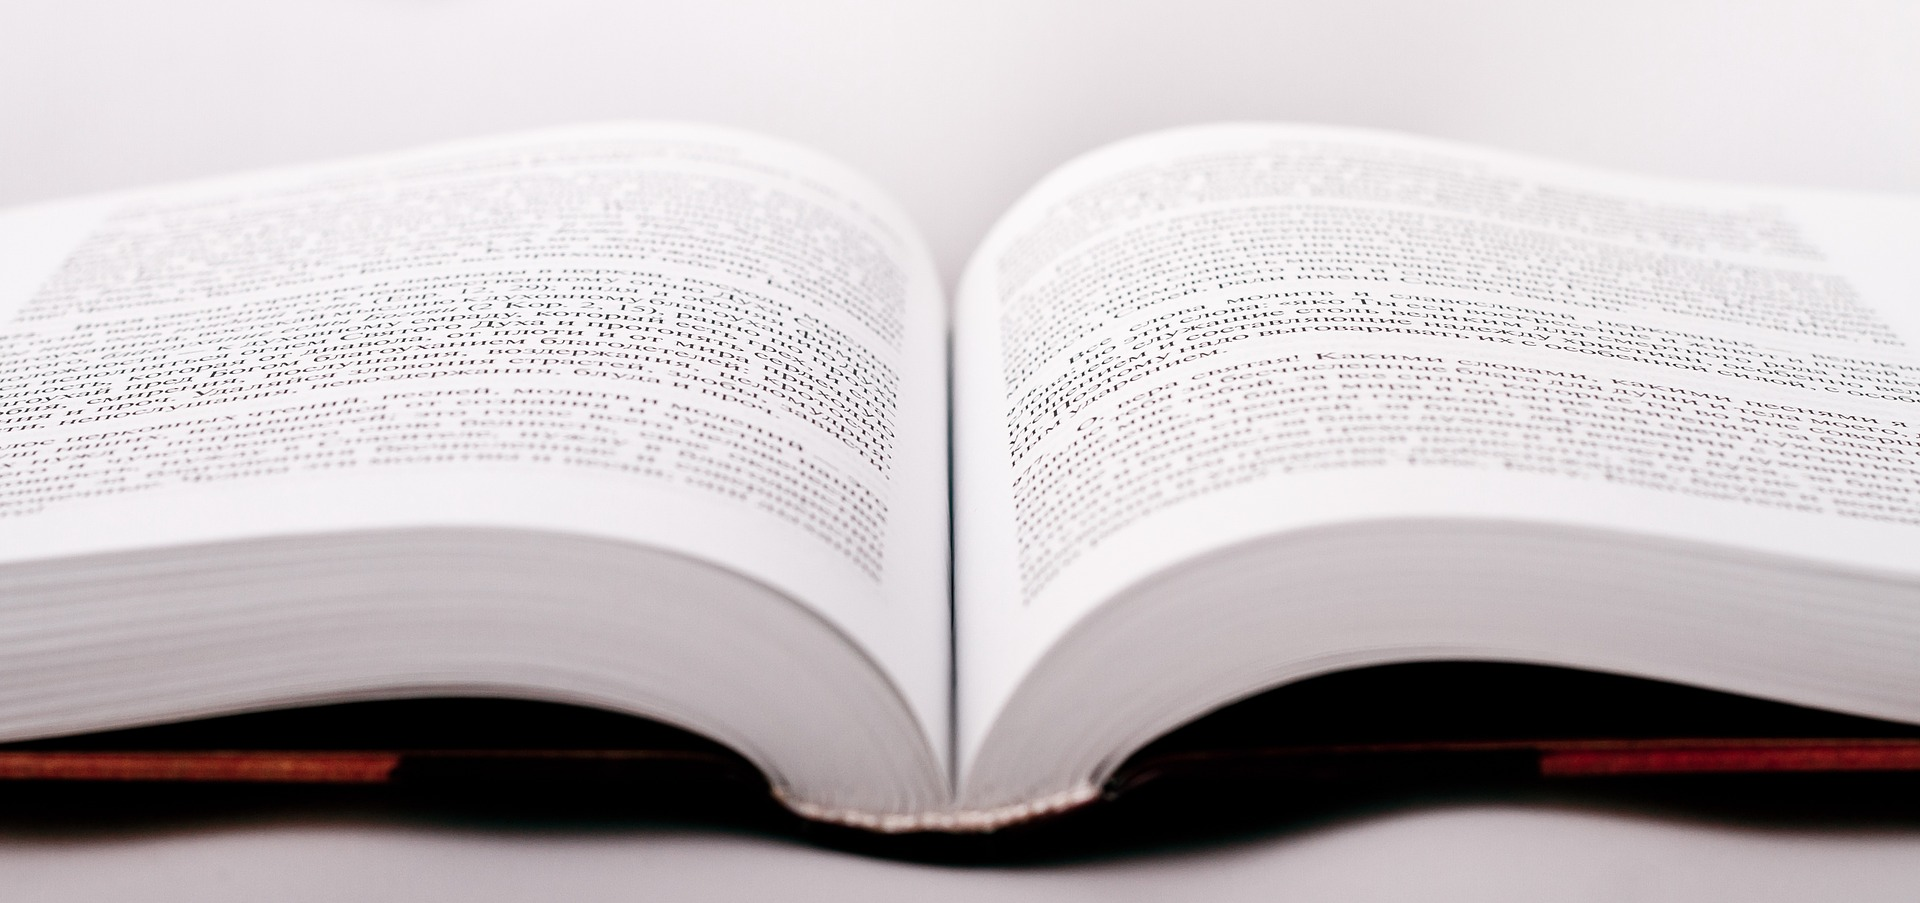
\includegraphics[width=1.5cm]{figs/bookpages}
  {\small \href{https://pixabay.com/en/book-reading-library-literature-1261800/}{Book}, by NikolayFrolochkin, Pixabay. \\ License: Creative Commons CC0\\}

\end{frame}



\frame{
~
\vspace{1cm}

\begin{flushright}


\includegraphics[width=2.2cm]{figs/by-sa}
 \\

\begin{footnotesize}
\copyright 2022 Jesus M. Gonzalez-Barahona. \\

\vspace{.4cm}

Some rights reserved. This document is distributed under the terms of the Creative Commons License ``Attribution-ShareAlike 4.0'',
available in \\
{\scriptsize \url{http://creativecommons.org/licenses/by-sa/4.0/}} \\

\vspace{.4cm}

This document (including source) is available from
\url{https://jgbarah.github.io/presentations}

\end{footnotesize}
\end{flushright}

}
%%

%\againframe{firstframe}

\end{document}

%%% Local Variables:
%%% mode: latex
%%% TeX-master: t
%%% End:
